
\section{Osnovne jednačine}

\begin{figure}[h!]
    \centering
    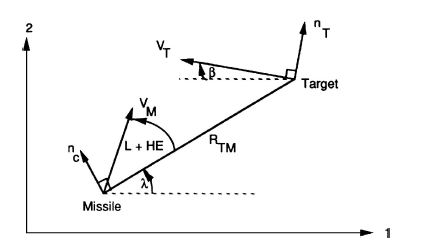
\includegraphics{PNfigure.JPG}
\end{figure}

Udaljenost između mete i projektila u svakom trenutku je data sa:
\begin{equation}
    r(t)=r_T(t)-r_M(t)
\end{equation}
Brzina približavanja projektila meti je data sa: 
\begin{equation}
    v_c=-\dot{r(t)}
\end{equation}

Ugaono ubrzanje mete je dato sa:
\begin{equation}
    \dot{\beta}=\frac{n_T}{v_T}
\end{equation}
Kompnente vektora brzine mete u koordinatnom sistemu vezanom za zemlju su date sa:
\begin{equation}
    v_{T1}=-v_T\cos{\beta}
\end{equation}
\begin{equation}
    v_{T2}=v_T\sin{\beta}
\end{equation}
Slično tome, brzina i ubrzanje projektila su date sa:
\begin{equation}
    \dot{v}_{M1}=a_{M1}
\end{equation}
\begin{equation}
    \dot{v}_{M2}=a_{M2}
\end{equation}
\begin{equation}
    \dot{R}_{M1}=v_{M1}
\end{equation}
\begin{equation}
    \dot{R}_{M2}=v_{M2}
\end{equation}

    \section{Izvođenje upravljačkog zakona}

%\subsection{SubSection Title}


